\documentclass[a5paper,12pt]{article}
\usepackage{../../../style}


\newcommand{\montitre}{Synchronisation }


\begin{document}

\fiche{Multiprogrammation}
\titre{Principes de la POO} : 
\begin{enumerate}
	\item Objet
	\item Méthode
	\item Classe
	\item Hiérarchie de classes
\end{enumerate}

\titre{Exemple : définition de la structure conditionnelle en smallTalk}\\
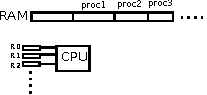
\includegraphics[width=180px]{Images/fig1.pdf}

\titre{Plan de cours}
\begin{enumerate}
	\item Introduction
	\item Concepts de base (objet, classe, envoi de message, hiérarchie)
	\item Illustrations et exemples (Java, Simula, SmallTalk
	\item Etude comparative de LO
	\item TP (Java, Eclipse)
\end{enumerate}

\titre{Histoire d'Ada}
Le département de la défense américain (Dod) est : 
\begin{itemize}
	\item Plus gros consommateur de logiciels
	\item 1968 - 73 : Le coût des SI augmente et le coût du matériel chute
	\item 73 : 7,5 milliards de dollars pour les Si
	\item 75 : 450 langages différents
	\item Réutilisabilité et partage de code inexistants
	\item 1983 : naissance d'Ada en réponse à la crise du logiciel et pour résoudre les pbs liés au dev de gros logiciels
	\item non issu d'un projet académique ou de recherche interne
\end{itemize}
Idée : Un seul langage incorporant tous les bons concepts de GL.\\

\titre{Paradigmes de programmation}
\begin{itemize}
	\item impérative
	\item fonctionnelle
	\item logique
	\item objet
	\item par contraintes
\end{itemize}

\newpage

\titre{Les domaines révolutionnés par la POO}
\begin{itemize}
	\item Génie logiciel (analyse, conception, programmation)
	\item Bases de données
	\item Intelligence artificielle (représentation des connaissances, programmation par agents)
\end{itemize}


\fiche{Processus et threads}
\titre{Fork :} Dans un systeme UNIX, les nouveaux processus sont toujours créés avec la commande fork(). 
\begin{itemize}
	\item Crée une nouvelle entrée dans la table des processus
	\item Copie de l'espace d'adressage
	\item Copie des descripteurs de fichiers
	\item Retourne
	\begin{itemize}
		\item 0 pour le fils
		\item un nombre positif strict pour le père
	\end{itemize}
\end{itemize}

\titre{Wait :} Le père devrait toujours attendre la fin de l'exécution de son fils avec la fonction waitpid, ou encore wait s'il n'a qu'un seul fils. \\

\titre{Thread :} Par défaut, un processus contient un unique thread (processus = ressource + un thread) \\ 
Créer un nouveau thread, c'est créer une nouvelle pile d'exécution à l'intérieur du même processus. \\ 

\titre{Création d'un thread :} On spécifie une fonction dont l'entête est \code{void* fct(void*)}\\

\titre{Figures correspondantes à la correction du td :}\\
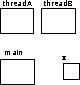
\includegraphics[width=100px]{fig3.pdf}
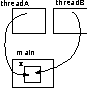
\includegraphics[width=100px]{fig4.pdf} \\\\
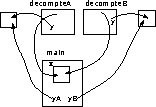
\includegraphics[width=200px]{fig5.pdf} \\\\
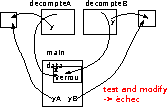
\includegraphics[width=200px]{fig6.pdf}



\fiche{Méthodes d'exclusion mutuelle}
\titre{Solution matérielle :} Le processus indique au CPU d'ignorer les interruptions. 
	\begin{itemize}
		\item Avantage : Plus de préemption imposée
		\item Inconvénients : Cette méthode est très dangereuse, elle compromet tout le système et exige de stopper tous les CPU.
	\end{itemize}

\titre{Solution logicielle 1 : L'alternance stricte} Variable "verrou" et attente active. Attention : "Test and Modify" ne marche pas. \\
\begin{minipage}{0.5\linewidth}
Algo A : \\
\\
Tantque vrai faire\\
  //section non critique\\
	Tantque verrou != 0 faire \\
		rien \\
	Fin Tantque\\
	verrou $\leftarrow$ 1\\
Fin Tantque\\
\end{minipage}
\begin{minipage}{0.5\linewidth}
Algo B : \\
\\
Tantque vrai faire\\
  //section non critique\\
	Tantque verrou != 1 faire \\
		rien \\
	Fin Tantque\\
	verrou $\leftarrow$ 0\\
Fin Tantque\\
\end{minipage}

\begin{itemize}
	\item Avantage : Simple, purement logiciel
	\item Inconvénient : Alternance stricte (pb résolu par Peterson), forte consommation CPU
\end{itemize}

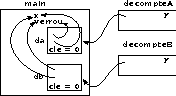
\includegraphics[width=200px]{fig7.pdf}

\titre{Définition :} Manipuler des objets définis par leurs caractéristiques externes (protocoles) indépendamment de toute représentation interne. \\

\titre{Deux manières de faire :}
\begin{itemize}
	\item Langage impératif + Constructions syntaxiques 
		\begin{itemize}
			\item regrouper les données et les programmes
			\item protéger (cacher, exporter)
			\item Séparer spécification et implémentation
			\item $\rightarrow$ on compte sur le bon sens du programmeur
			\item exemples : ADA, Pascal
		\end{itemize}
	\item Langage objet
		\begin{itemize}
			\item Définir de nouveaux types, et les manipuler (c'est la manipulation qui fait la différence avec les langages impératifs)
			\item Différence entre les types prédéfinis et types utilisateurs (ne devrait pas exister dans un langage purement objet)
			\item exemples : Simula67, SmallTalk80, Common Lisp objet, Eiffel, C++, Java, Objective C, Ruby, Python, C\#, Groovy, Lisaac
		\end{itemize}
\end{itemize}

\titre{Type abstrait :}
\begin{itemize}
	\item Données
	\item Opérateurs
	\item Propriétés
\end{itemize}

\titre{Caractéristiques}
\begin{itemize}
	\item Modularité
	\item Sécurité
	\item Spécification
	\item Réutilisabilité
\end{itemize}

\titre{Exemple :} Pile d'entiers
\begin{itemize}
	\item Pile, Entier, Booléen
	\item 
		\begin{itemize}
			\item pile\_vide : Pile $\rightarrow$ Booléen
			\item empiler : Pile $\times$ Entier $\rightarrow$ Pile
			\item depiler : Pile $\rightarrow$ Piles $\times$ Entier
		\end{itemize}
	\item
		\begin{itemize}
			\item non(pile\_vide(empiler(p,e)))
			\item depiler(empiler(p,e)) = (p,e)
			\item non(pile\_vide(p)) $\impl$ empiler(depiler(p)) = p
		\end{itemize}
\end{itemize}

\titre{Approche descriptive}
\begin{itemize}
	\item La réalité est composée d'objets (perçu, concret, animé ou non, conçu, abstrait) $\rightarrow$ connaissance singulière
	\item Caractéristiques contingentes (peu varier) $\rightarrow$ attributs
	\item Caractéristiques essentielles (intrinsèque) $\rightarrow$ classes différentes
	\item Objet $\rightarrow$ Concept (abstraction de classes : fox $\rightarrow$ voiture $\rightarrow$ moyen de locomotion)
	\item Concept $\rightarrow$ Exemplification (spécialisation de classe : moyen de locomotion $\rightarrow$ voiture $\rightarrow$ fox
\end{itemize}

\titre{Approche service (fonctionnelle) :} Objet $\equiv$ Composant. L'accent est mis sur les caractéristiques externes, descriptives et comportementales de l'objet. \\ \\
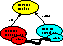
\includegraphics[width=150px]{Images/fig2.pdf} \hspace{1cm}
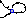
\includegraphics[width=150px]{Images/fig3.pdf} \\
\begin{itemize}
	\item Encapsulation des données, boite noire
	\item Un objet permet de regrouper en une seule entité et de façon indissociable données et procédures d'exploitation.
	\item Un objet est une instance de classe 
		\begin{itemize}
			\item ses données sont les variables d'instance, attributs variables, données membres. Les données sont accessibles uniquement à traver les procédures (programmation par état) $\rightarrow$ c'est rémanent (ie si l'objet se modifie lors d'une procédure, alors l'état initial n'est pas restauré). \\
			Remarque : En Java, l'unité d'encapsulation est la classe (les objets d'une même classe peuvent accéder aux champs privés des autres instances de la même classe). Ca devrait être l'objet.
			\item Les procédures sont les méthodes, attributs procédures, fonctions membres. Il y a des méthodes exportées (elles définissent l'interface) et des méthodes cachées (utiles uniquement à l'implémentation)
		\end{itemize}
\end{itemize}

\titre{Programmation par état :}
	\begin{itemize}
		\item On travaille par référence et non par valeur
		\item En java, les types primitifs passent par valeur
	\end{itemize}

\titre{Exemple :} Processus
\begin{itemize}
	\item Que \titre{fait} un processus ?
	\begin{itemize}	
		\item Suspendre
		\item Réveiller
		\item Priorité
	\end{itemize}
	\item Qu'\titre{est} un processus ? 
	\begin{itemize}
		\item Ressources
		\item Contexte
		\item Programme
	\end{itemize}
	\item $\rightarrow$ Ces deux points de vue peuvent être mixés par l'héritage multiple, mais nous en général on choisira une des deux approches et on s'y tiendra.
\end{itemize}


\fiche{TD1}
\titre{question 1} \\ Exemple basique de fork : une variable est dupliquée du père au fils. \\
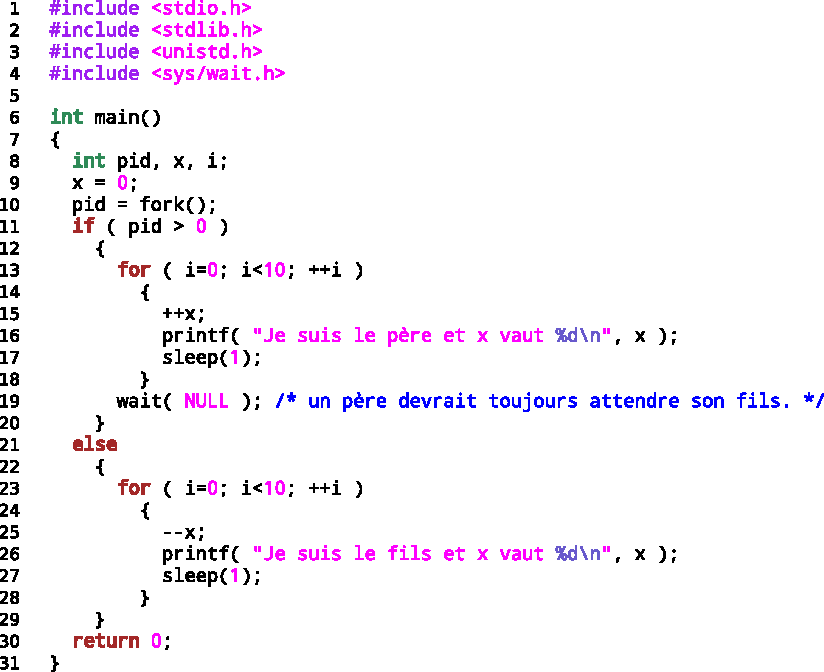
\includegraphics[width=\linewidth]{fig25.pdf}\newpage
\titre{question 2}
\begin{enumerate}
	\item Deux threads manipulent la même variable globale \\
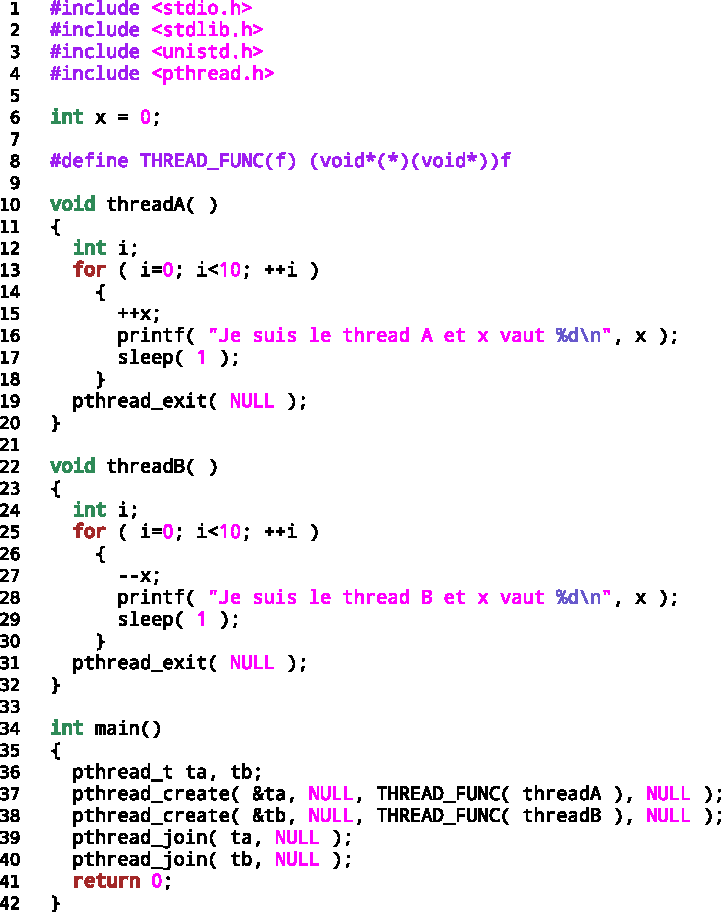
\includegraphics[width=\linewidth]{fig26.pdf}\newpage
	\item Deux threads manipulent la même variable grâce aux pointeurs \\
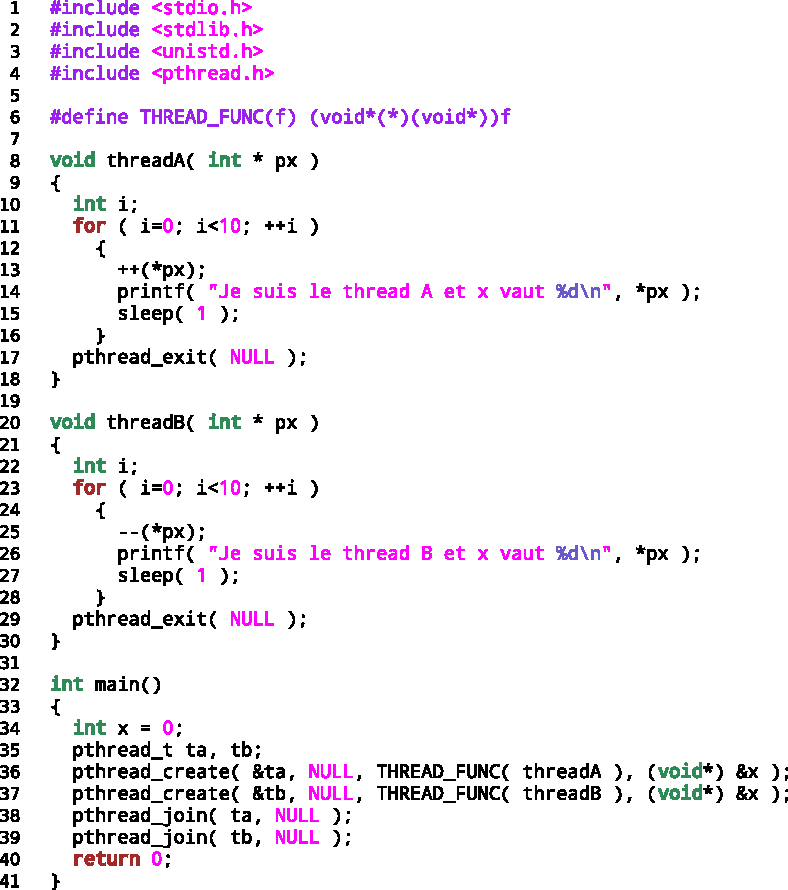
\includegraphics[width=\linewidth]{fig27.pdf}\\
\end{enumerate} \newpage
\titre{question 3}
\begin{enumerate}
	\item Deux threads décrémentent un même variable\\
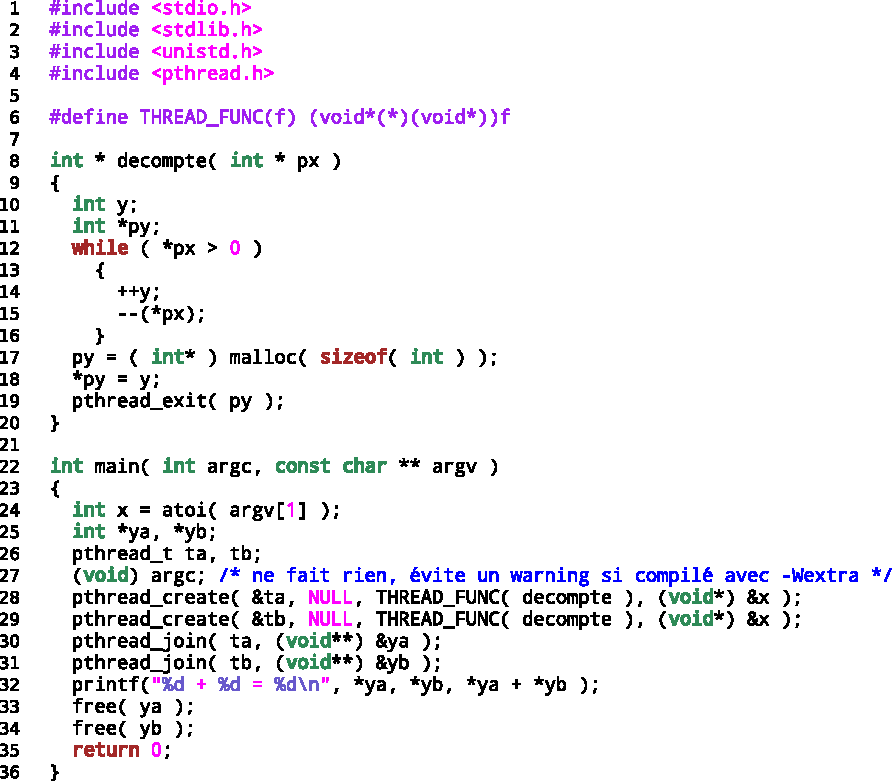
\includegraphics[width=\linewidth]{fig28.pdf}\newpage
	\item Nous essayons d'utiliser un verrou pour éviter les problèmes de concurrence (attente active)\\
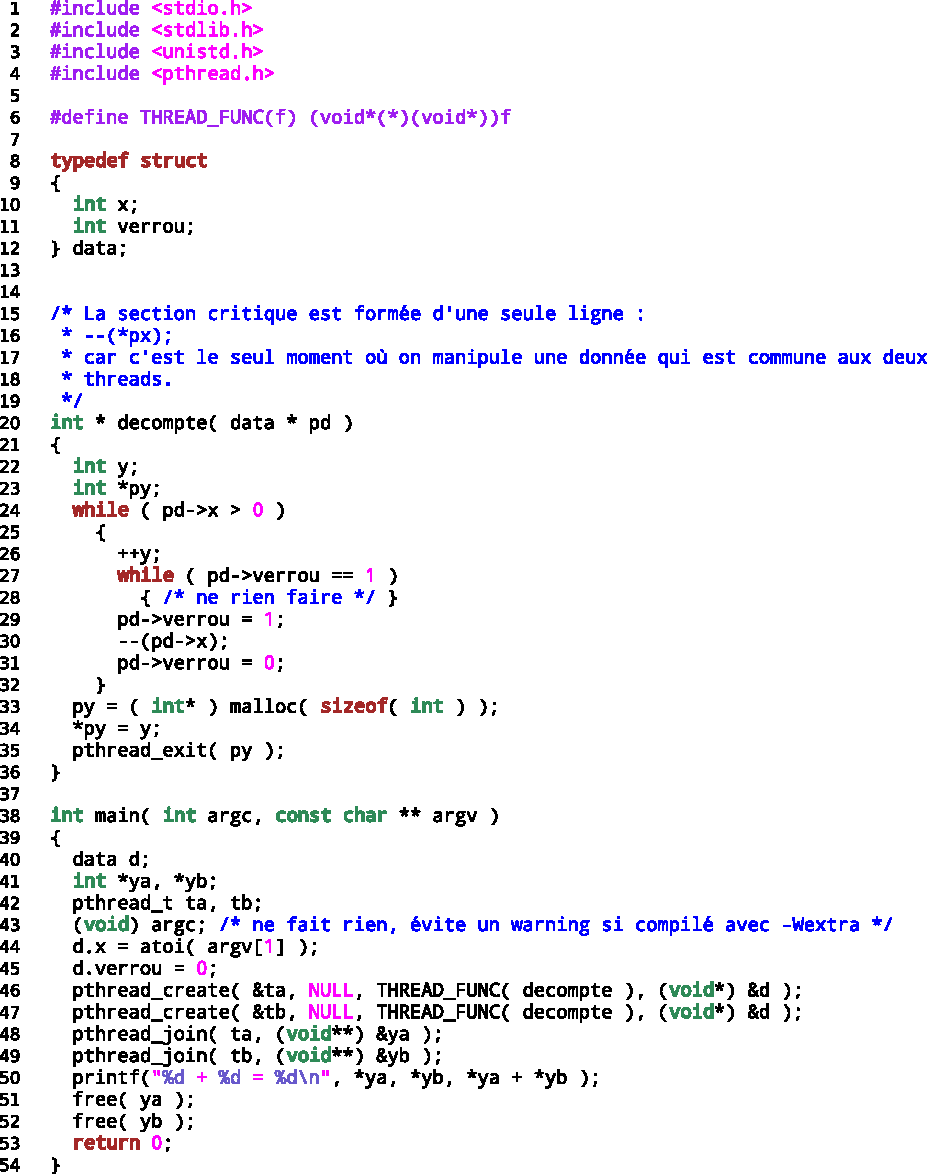
\includegraphics[width=\linewidth]{fig29.pdf}\\
\end{enumerate}


\fiche{TD2}
\titre{Exercice 1 :}
\begin{enumerate}
	\item Condition de concurrence : le résultat final dépend de l'ordonnancement
	\item Section critique : portion de code où deux processus ne devraient jamais se trouver en même temps sous peine de créer une condition de concurrence.
\end{enumerate}

\titre{Exercice 2}
\begin{enumerate}
	\item La création d'un thread est plus rapide que la création d'un processus.
	\item Pour être le plus général possible. Pour plusieurs variables on crée une struct. (idée : créer une fonction bidon qui va répartir les champs de la struct en argument et appeler la fonction qu'on veut)
	\item Il sert à enregistrer le retour d'une fonction.
	\item La valeur renvoyée par pthread\_join et pthread\_create est 0 pour un succès, autre chose pour une erreur.
\end{enumerate}

\titre{Exercice 3}
\begin{enumerate}
	\item 1,5 secondes
	\item 15 + 100*75 = 7515
	\item 100*15 + 10*75 = 2250 \\ 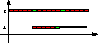
\includegraphics[width=200px]{fig8.pdf}
	\item 1,5 secondes \\ 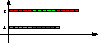
\includegraphics[width=200px]{fig9.pdf}
\end{enumerate}

\titre{Exercice 4}
\begin{enumerate}
	\item Un thread peut s'activer sur les requetes en cache pendant qu'un autre attend le disque dur
	\item L'appel à pthread\_create échouera si on dépasse le nombre maximal de thread autorisé
	\item  .\\ 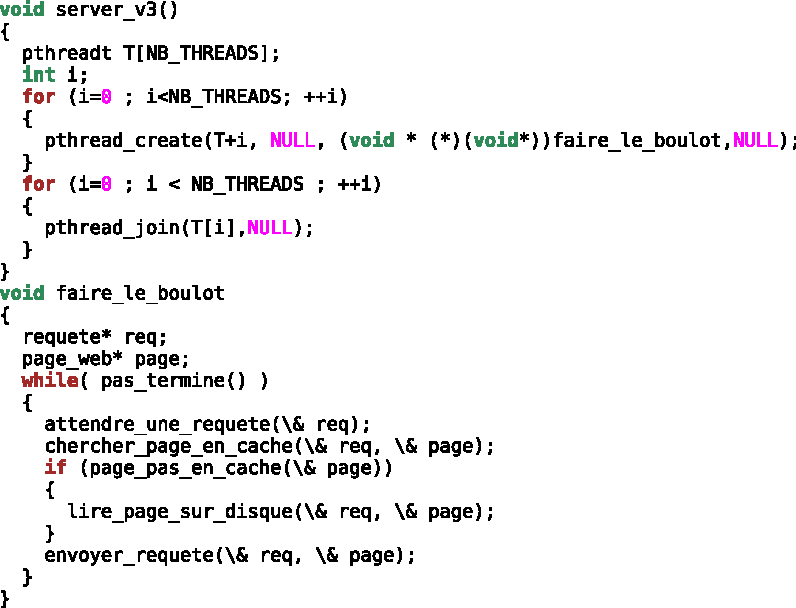
\includegraphics[width=300px]{fig10.pdf}

\end{enumerate}

\titre{Exercice 5 :} 
\begin{enumerate}
	\item $A1, A2, A3, A4, A5, B1, B2, B3, B4, B5, B6, B7, A6, A7$
	\item La section critique est composée des lignes 4 à 6
	\item Inverser les lignes 5 et 6 (la copie du document n'a pas besoin d'être en section critique.
\end{enumerate}

\titre{Exercice 6 :} \\
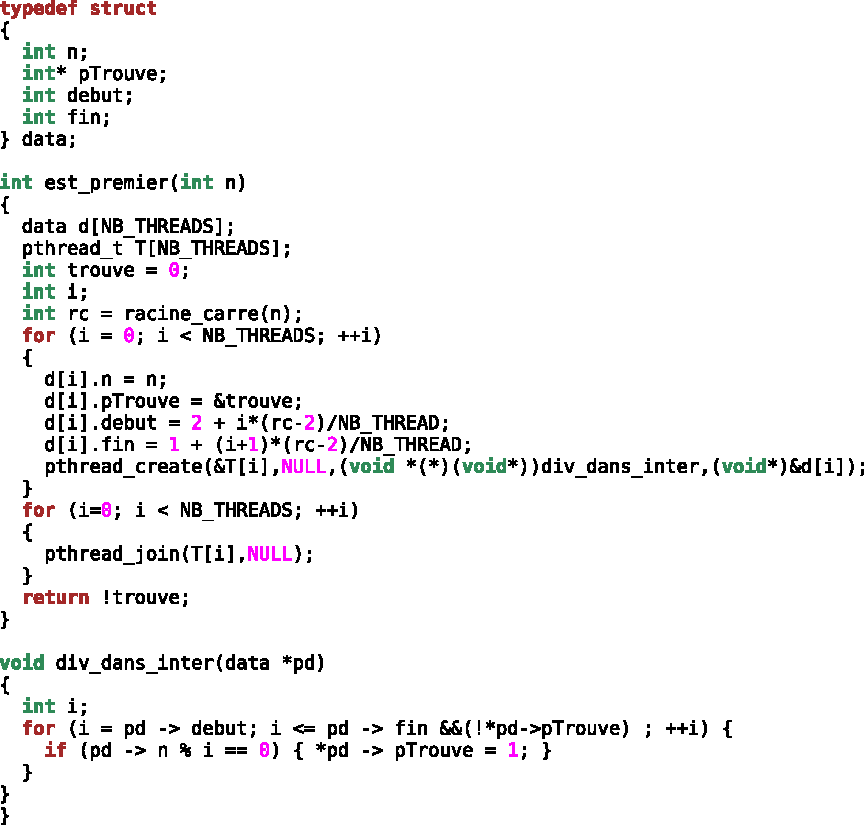
\includegraphics[width=300px]{fig11.pdf}


\fiche{TD3}
\input{2901.tex}

\fiche{Mémoire partagée}
\titre{Principe :} Avoir des pages de mémoire inscrites dans l'espace d'adressage de plusieurs processus.\\
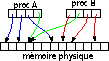
\includegraphics[width=200px]{fig19.pdf}

\titre{Avantage :} C'est le moyen le plus rapide d'échanger des données entre deux processus.\\

\titre{Inconvénient :} C'est aussi un très bon moyen pour créer des conditions de concurrence.\\

\titre{Comment ça marche ?} 
\begin{enumerate}
	\item Un processus crée un fichier virtuel (shm\_open)
	\item On redimensionne le fichier à la taille voulue (ftruncate)
	\item Projeter le fichier virtuel dans l'espace d'adressage du processus (mmap)
	\item Les processus qui veulent l'utiliser ouvrent le fichier (shm\_open) et le projettent dans leur espace d'adressage (mmap)
	\item Les processus utilisent cette mémoire partagée (attention aux conditions de concurrence)
	\item Lorsqu'un processus a terminé il ferme la projection (munmap) et le fichier (fclose)
	\item Lorsque tous les processus ont terminé, on détruit le fichier (shm\_unlink)
\end{enumerate}


\fiche{Exo Fork et mémoire partagée}
\titre{Exemple prof :}  Le processus mp1 crée un espace partagé de la taille d'un entier et demande en boucle à l'utilisateur de changer la valeur de cet entier. Le processus mp2 utilise cet espace partagé et affiche en boucle la valeur de l'entier toutes les secondes. \\

\titre{Modifications apportées pour tester ce qu'il se passe lors d'un fork :} Je n'ai pas modifié le fichier mp1. Par contre dans le fichier mp2 j'ai fait un fork avant d'entrer dans la boucle, puis dans la boucle, le processus indique s'il est le père ou le fils avant d'afficher la valeur de l'entier.\\

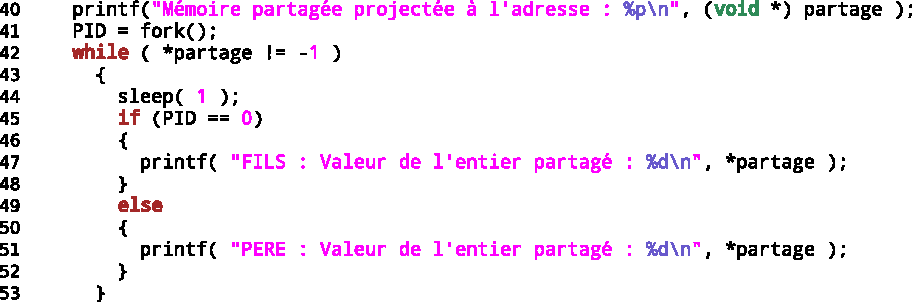
\includegraphics[width=\linewidth]{fig21.pdf}

\titre{Conclusion :} On pouvait naturellement imaginer que les deux processus allaient reconnaitre la valeur de l'entier partagé. En effet, la mémoire est copiée du père au fils, et l'espace mémoire mappé est donc copié avec son mapping, donc dans le fils le mapping vers le fichier virtuel existe toujours. C'est bien ce résultat attendu qui s'est produit. \\

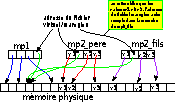
\includegraphics[width=\linewidth]{fig20.pdf}\\

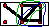
\includegraphics[width=\linewidth]{fig22.pdf}


\fiche{Variables de condition}
\titre{Scénario classique :} \\
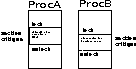
\includegraphics[width=300px]{fig32.pdf}\\

\titre{Utilisation :} Une \titre{Variable de condition} s'utilise toujours de paire avec un mutex. \\

\titre{3 primitives :}
\begin{enumerate}
	\item cond\_wait(C: Variable de condition, M:Mutex). Doit être appelé à l'intérieur d'une section critique protégée par M. Ce que ça fait :
	\begin{enumerate}	
		\item unlock(M)
		\item attendre un signal sur C
		\item lock(M)
	\end{enumerate}
	Intérêt de l'appel système pour faire ça : le passage de a à b est atomique, tout comme le passage entre b et c.
	\item cond\_signal(C: Variable de condition) Débloque au moins un processus bloqué sur C.
	\item cond\_broadcast(C: Variable de condition) Débloque tous les processus bloqués sur C.
\end{enumerate}

\titre{Remarque :} 
\begin{enumerate}
	\item Les variables de condition sont sans mémoire. Un signal émis lorsqu'aucun processus n'est en attente est perdu.
	\item Un cond\_wait s'exécute toujours à l'intérieur d'un tantque.
\end{enumerate} 

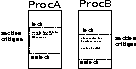
\includegraphics[width=300px]{fig33.pdf}\newpage

\titre{Producteurs/consommateurs :}\\
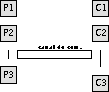
\includegraphics[width=200px]{fig34.pdf}\\


\fiche{Barrières de synchronisation}
\titre{Exemple :} NoeudPersonne hérite de Noeud(méthodes de gestion d'un noeud), et de Personne(méthodes de gestion d'une personne. Si l'héritage multiple n'est pas géré, on peut hériter de Noeud uniquement avec une instance de Personne, ou utiliser un objet composite avec un attribut Noeud et un attribut Personne.\\

\titre{Problème :} Définir un sous-concept à partir de plusieurs sur-concepts a-t-il un sens ?


\fiche{Tubes}
\titre{Règle :} Seules les classes terminales peuvent être instanciées. Toute classe possédant des spécialisations est une classe abstraite (ne peut être instanciée). Les extensions des classes terminales d'une classe générique constituent une partition de l'ensemble des instances relevant de la classe générique (classe de base, abstraite).


\fiche{Problèmes liés à la synchronisation}
\titre{Resource :} Objet physique ou virtuel pouvant être alloué à un seul processus à la fois.\\

\titre{Resources retirables :} Peut être retirée au processus, utilisé par un autre, puis rendu au premier sans compromettre son exécution (exemples : CPU, RAM). \\

\titre{Resources non retirables :} Ne peut être retirée au processus que lorsqu'il en aura décidé. \\

\titre{3 étapes pour accéder à une resource non retirable :}
\begin{enumerate}
	\item Solliciter la resource
	\item Utiliser la resource
	\item Libérer la resource
\end{enumerate}

\titre{Famine :} Situation où un processus demande l'accès à une ressource mais ne l'obtient jamais car elle est toujours attribuée à d'autres processus.\\

\titre{Solution :} Le principe FIFO permet d'éviter la famine mais n'est pas toujours souhaitable. \\

\titre{Interblocage :} Situation où un ensemble de processus attendent un événement que seul un des processus de l'ensemble peut provoquer.\\

\titre{Exemple :}\\
\begin{tabular}{l|l}
Proc A & Proc B \\ \hline
Lock(M1) & Lock(M2) \\ 
Lock(M2) & Lock(M1) \\
\ldots & \ldots \\
Unlock(M2) & Unlock(M1) \\
Unlock(M1) & Unlock(M2) \\
\end{tabular}

\titre{Modélisation du problème : Modèle de Holt } (1972) On trace le graphe des attentes qui contient deux types de sommets (carré = ressource, rond = processus) \\
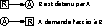
\includegraphics[width=100px]{fig37.pdf}\\

\titre{Exemple :}\\
\begin{tabular}{l|l|l}
A & B & C \\ \hline
D(R) & D(S) & D(T) \\
D(S) & D(T) & D(R) \\
L(R) & L(S) & L(T) \\
L(S) & L(T) & L(R) \\
\end{tabular} \\
Si l'ordonnancement est A,B,C,A,C on obtient : \\
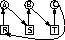
\includegraphics[width=100px]{fig38.pdf} \\

\titre{Stratégie face aux interblocages}
\begin{enumerate}
	\item Les ignorer
	\item Les détecter et y remédier 
	\begin{itemize}
		\item Mettre à jour dynamiquement le graphe des attentes lancer périodiquement un algo de détection des cycles. En cas d'interblocage on tue un des processus et on libère toutes ses ressources.
	\end{itemize}
	\item Détecter dynamiquement si il est sûr d'allouer une ressource
	\begin{itemize}
		\item 
		\begin{tabular}{l|l}
			A & B \\ \hline
			D(R) & D(S) \\
			D(S) & D(R) \\
			L(R) & L(S) \\
			L(S) & L(R) \\
		\end{tabular} \\
		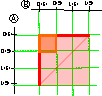
\includegraphics[width=100px]{fig39.pdf} \\
		On appelle état sûr un état à partir duquel on peut exécuter tous les processus un après l'autre dans un certain ordre sans qu'aucun ne soit bloqué. Un interblocage survient toujours à partir d'un état non sûr. \\ Pour déterminer les états sûrs, il faut connaitre à l'avance le code que vont exécuter les programmes. 
	\end{itemize}
	\item Imposer des contraintes pour s'assurer qu'un interblocage est impossible
	\begin{itemize}
		\item Pas d'exclusion mutuelle
		\item Ordonne les ressources
	\end{itemize}
\end{enumerate}


\end{document}
